\documentclass[12pt]{article}
\usepackage[margin=1in]{geometry} 
\usepackage{amsmath}
\usepackage{amssymb}
\usepackage{amsthm}
\usepackage{accents}
\usepackage{graphicx}


\setlength{\oddsidemargin}{0in}
\setlength{\textwidth}{6.5in}
\setlength{\topmargin}{-.55in}
\setlength{\textheight}{9in}
\pagestyle{empty}
\renewcommand \d{\displaystyle}
\renewcommand \a{\shortstack{$\rightarrow$\\$u$}}
\renewcommand \b{\shortstack{$\rightarrow$\\$v$}}

\begin{document}
\noindent Math 5510

\noindent Topology

\noindent Stephanie Klumpe

\vspace{.2in}
\begin{center}
Problem Set 7
\end{center}

 \begin{enumerate}%\setlength{\itemindent}{-1.5em}
\item (\#1 in 5.4) Sketch some open sets in the quotient space $\mathbb{R}/\sim$ of Example 5.2. (If you are writing your solutions in LaTeX, you may sketch these on paper, scan and email them to me, or upload in Canvas as a second file). Be sure to show that the sets in $\mathbb{R}_{\mathcal{U}}$ that project to these sets under the quotient map $\nu: \mathbb{R}\to \mathbb{R}/\sim$.\\\\
For ease of writing, we will denote the projection of an interval $(a,b)\in\mathbb{R}$ by $([a],[b])$.
\begin{center}
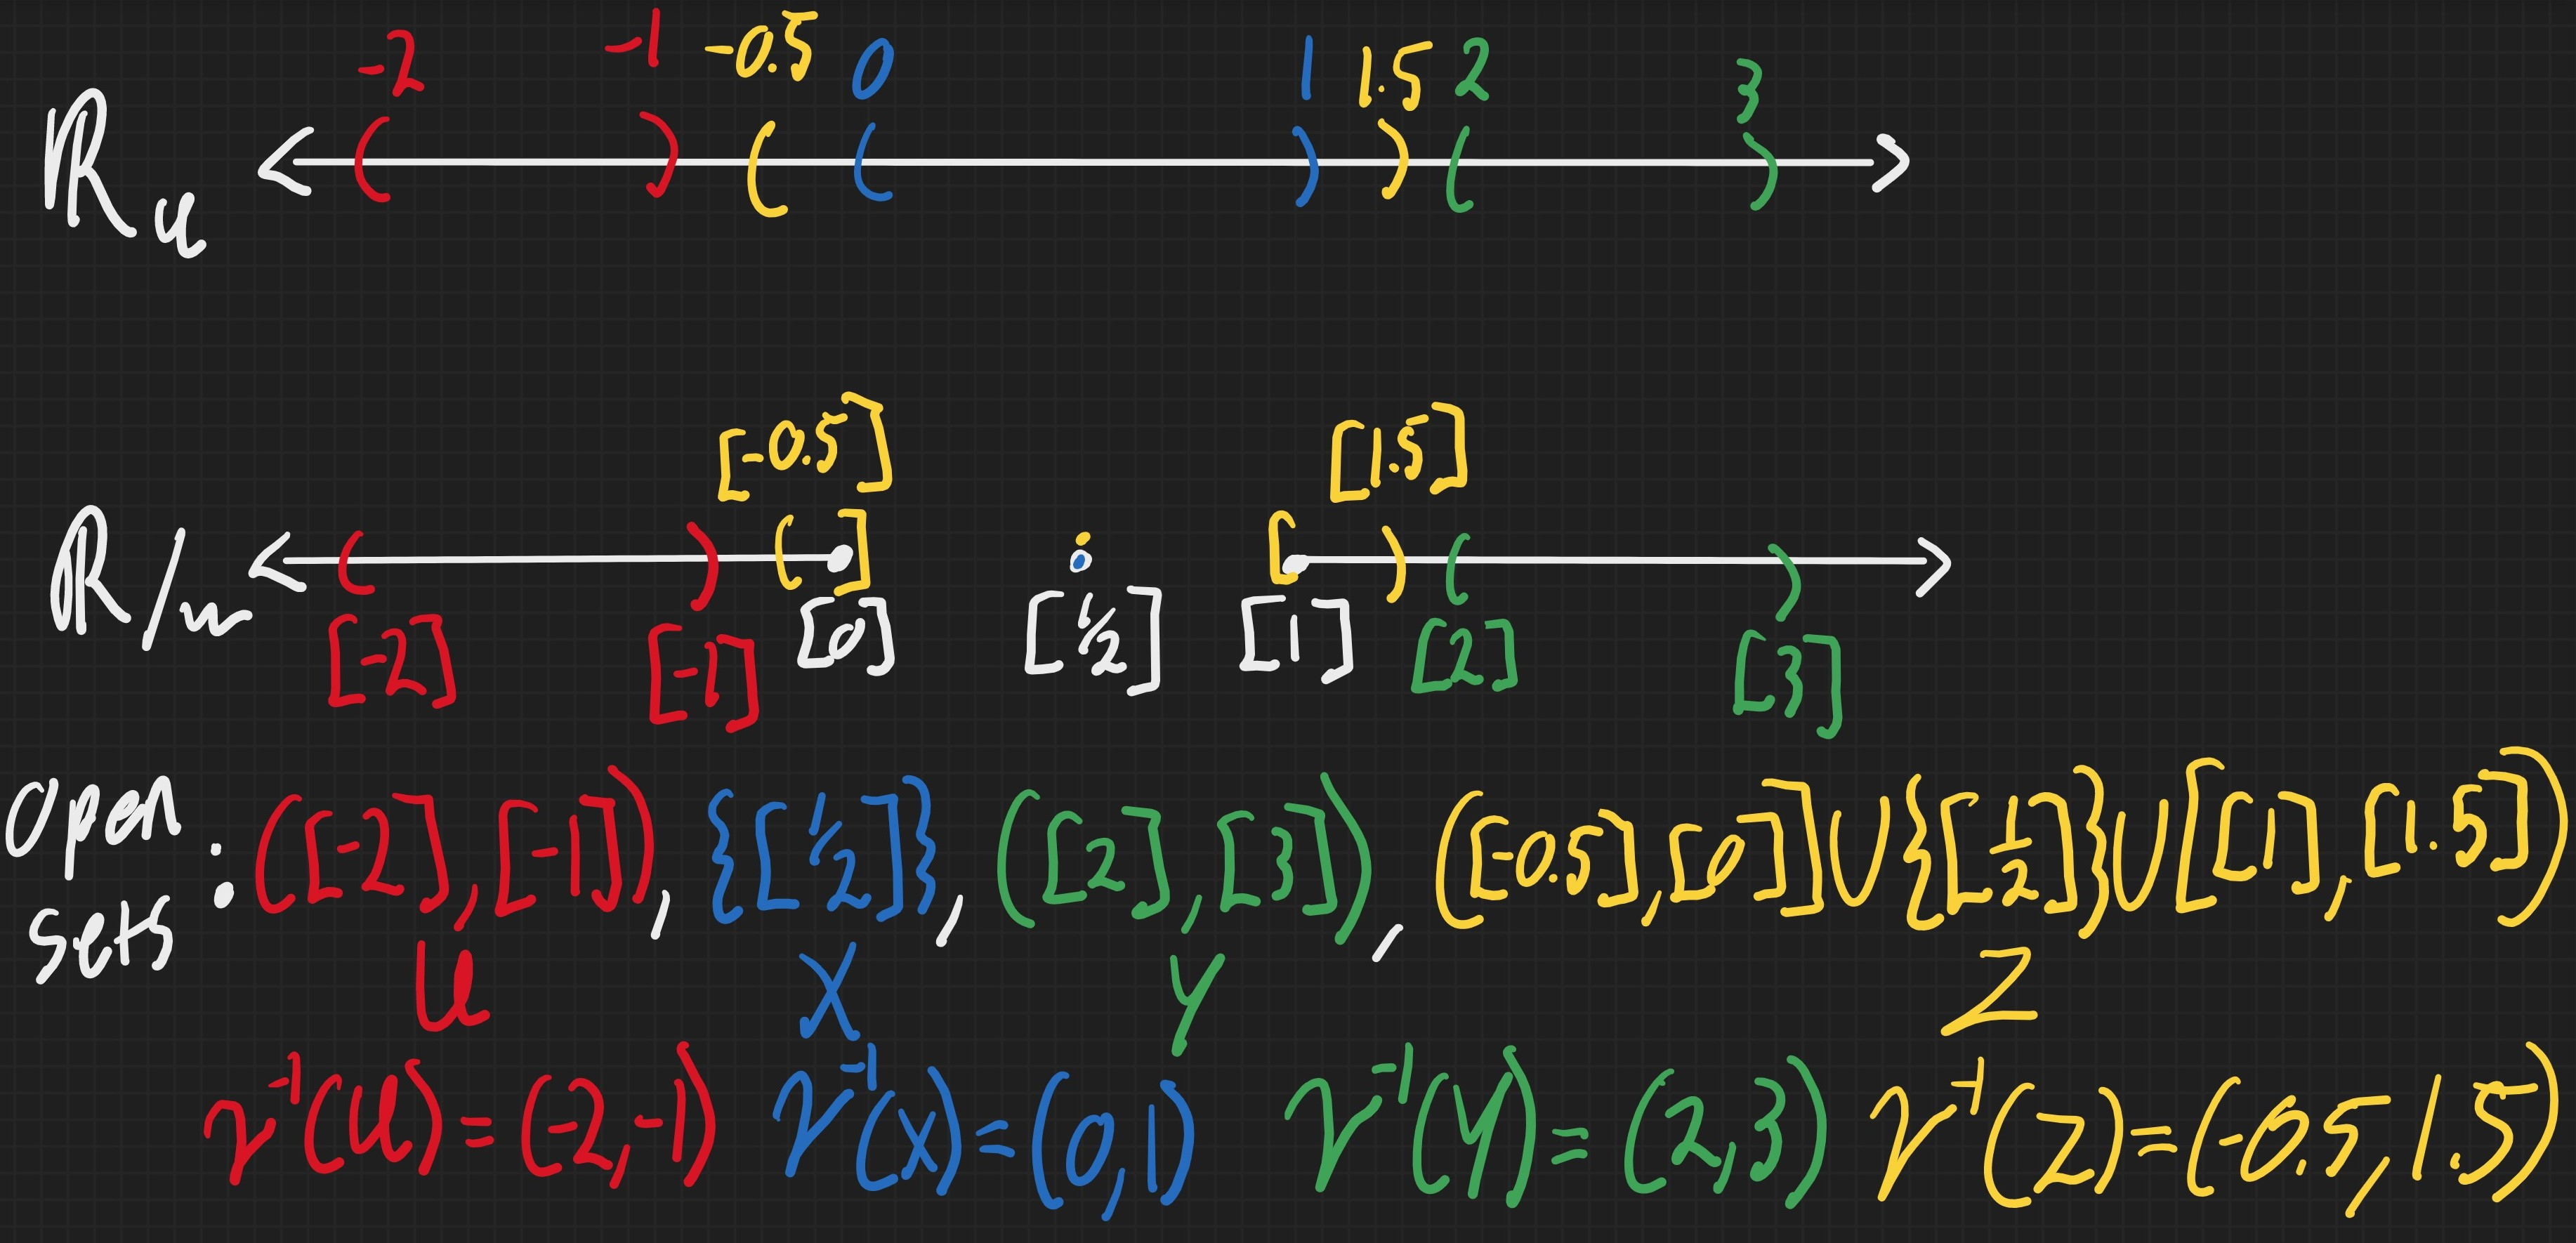
\includegraphics[scale=0.4]{ps7p1.JPG}
\end{center}
\item Find a subspace $X$ of $\mathbb{R}^2$ and an equivalence relation $\sim$ on $X$ so that $X/\sim\cong S^2$, where $S^2$ is the unit sphere centered at the origin in $\mathbb{R}^3$. Illustrate typical open sets in the quotient space and in $X$. You do not have to give an explicit homeomorphism between $X/\sim$ and $S^2$, but you should describe a function between the two and explain why it is a homeomorphism.\\\\
Consider the set $D=\{(x,y)\in\mathbb{R}^2|x^2+y^2\leq1\}$ and define $\sim$ by $(x_1,y_1)\sim(x_2,y_2)$ if $\sqrt{x_1^2+y_1^2}=\sqrt{x_2^2+y_2^2}=1$, and $(x,y)\sim(x,y)$ otherwise. Then we have that $D/\sim\cong S^2$. The function that is a homeomorphism, $f$, takes each point on $D/\sim$ and maps it to a unique point on the unit sphere. $f$ also maps to every point on $S^2$. In particular, $f$ maps points in $D/\sim$ that are given by $x^2+y^2<1$ to some point on the surface of $S^2$ and the points given by $x^2+y^2=1$ are mapped to the 'pole' of $S^2$ as shown below. For example, $(0,0)$ maps to the point $(0,0,-1)$ since each point on $S^2$ is a distance of one form $(0,0,0)$. Another example would be $(0,1)$ would map to $(0,0,1)$ by the same logic due to the equivalence relation. Also, the point $(0,\frac12)$ on the cicrle of radius $\frac12$ would map to $(0,\frac12,\sqrt{\frac34})$ so that the point is a distance of one away fro the origin in $\mathbb{R}^3$. So, every concentric circle of radius $\epsilon<1$ would map to some circle on $S^2$ such that the $z$ coordinate would be $z^2=1-x_{\epsilon}^2-y_{\epsilon}^2$ where $x_{\epsilon},y_{\epsilon}$ are points on the circle of radius $\epsilon$. Now in particular, $f$ maps open surface patches on $D/\sim$ to open patches on $S^2$. Similarly, $f^{-1}$ maps open patches on $S^2$ to open patches on $D/\sim$. Example open sets on both $D$ and $D/\sim$ are given below.
\begin{center}
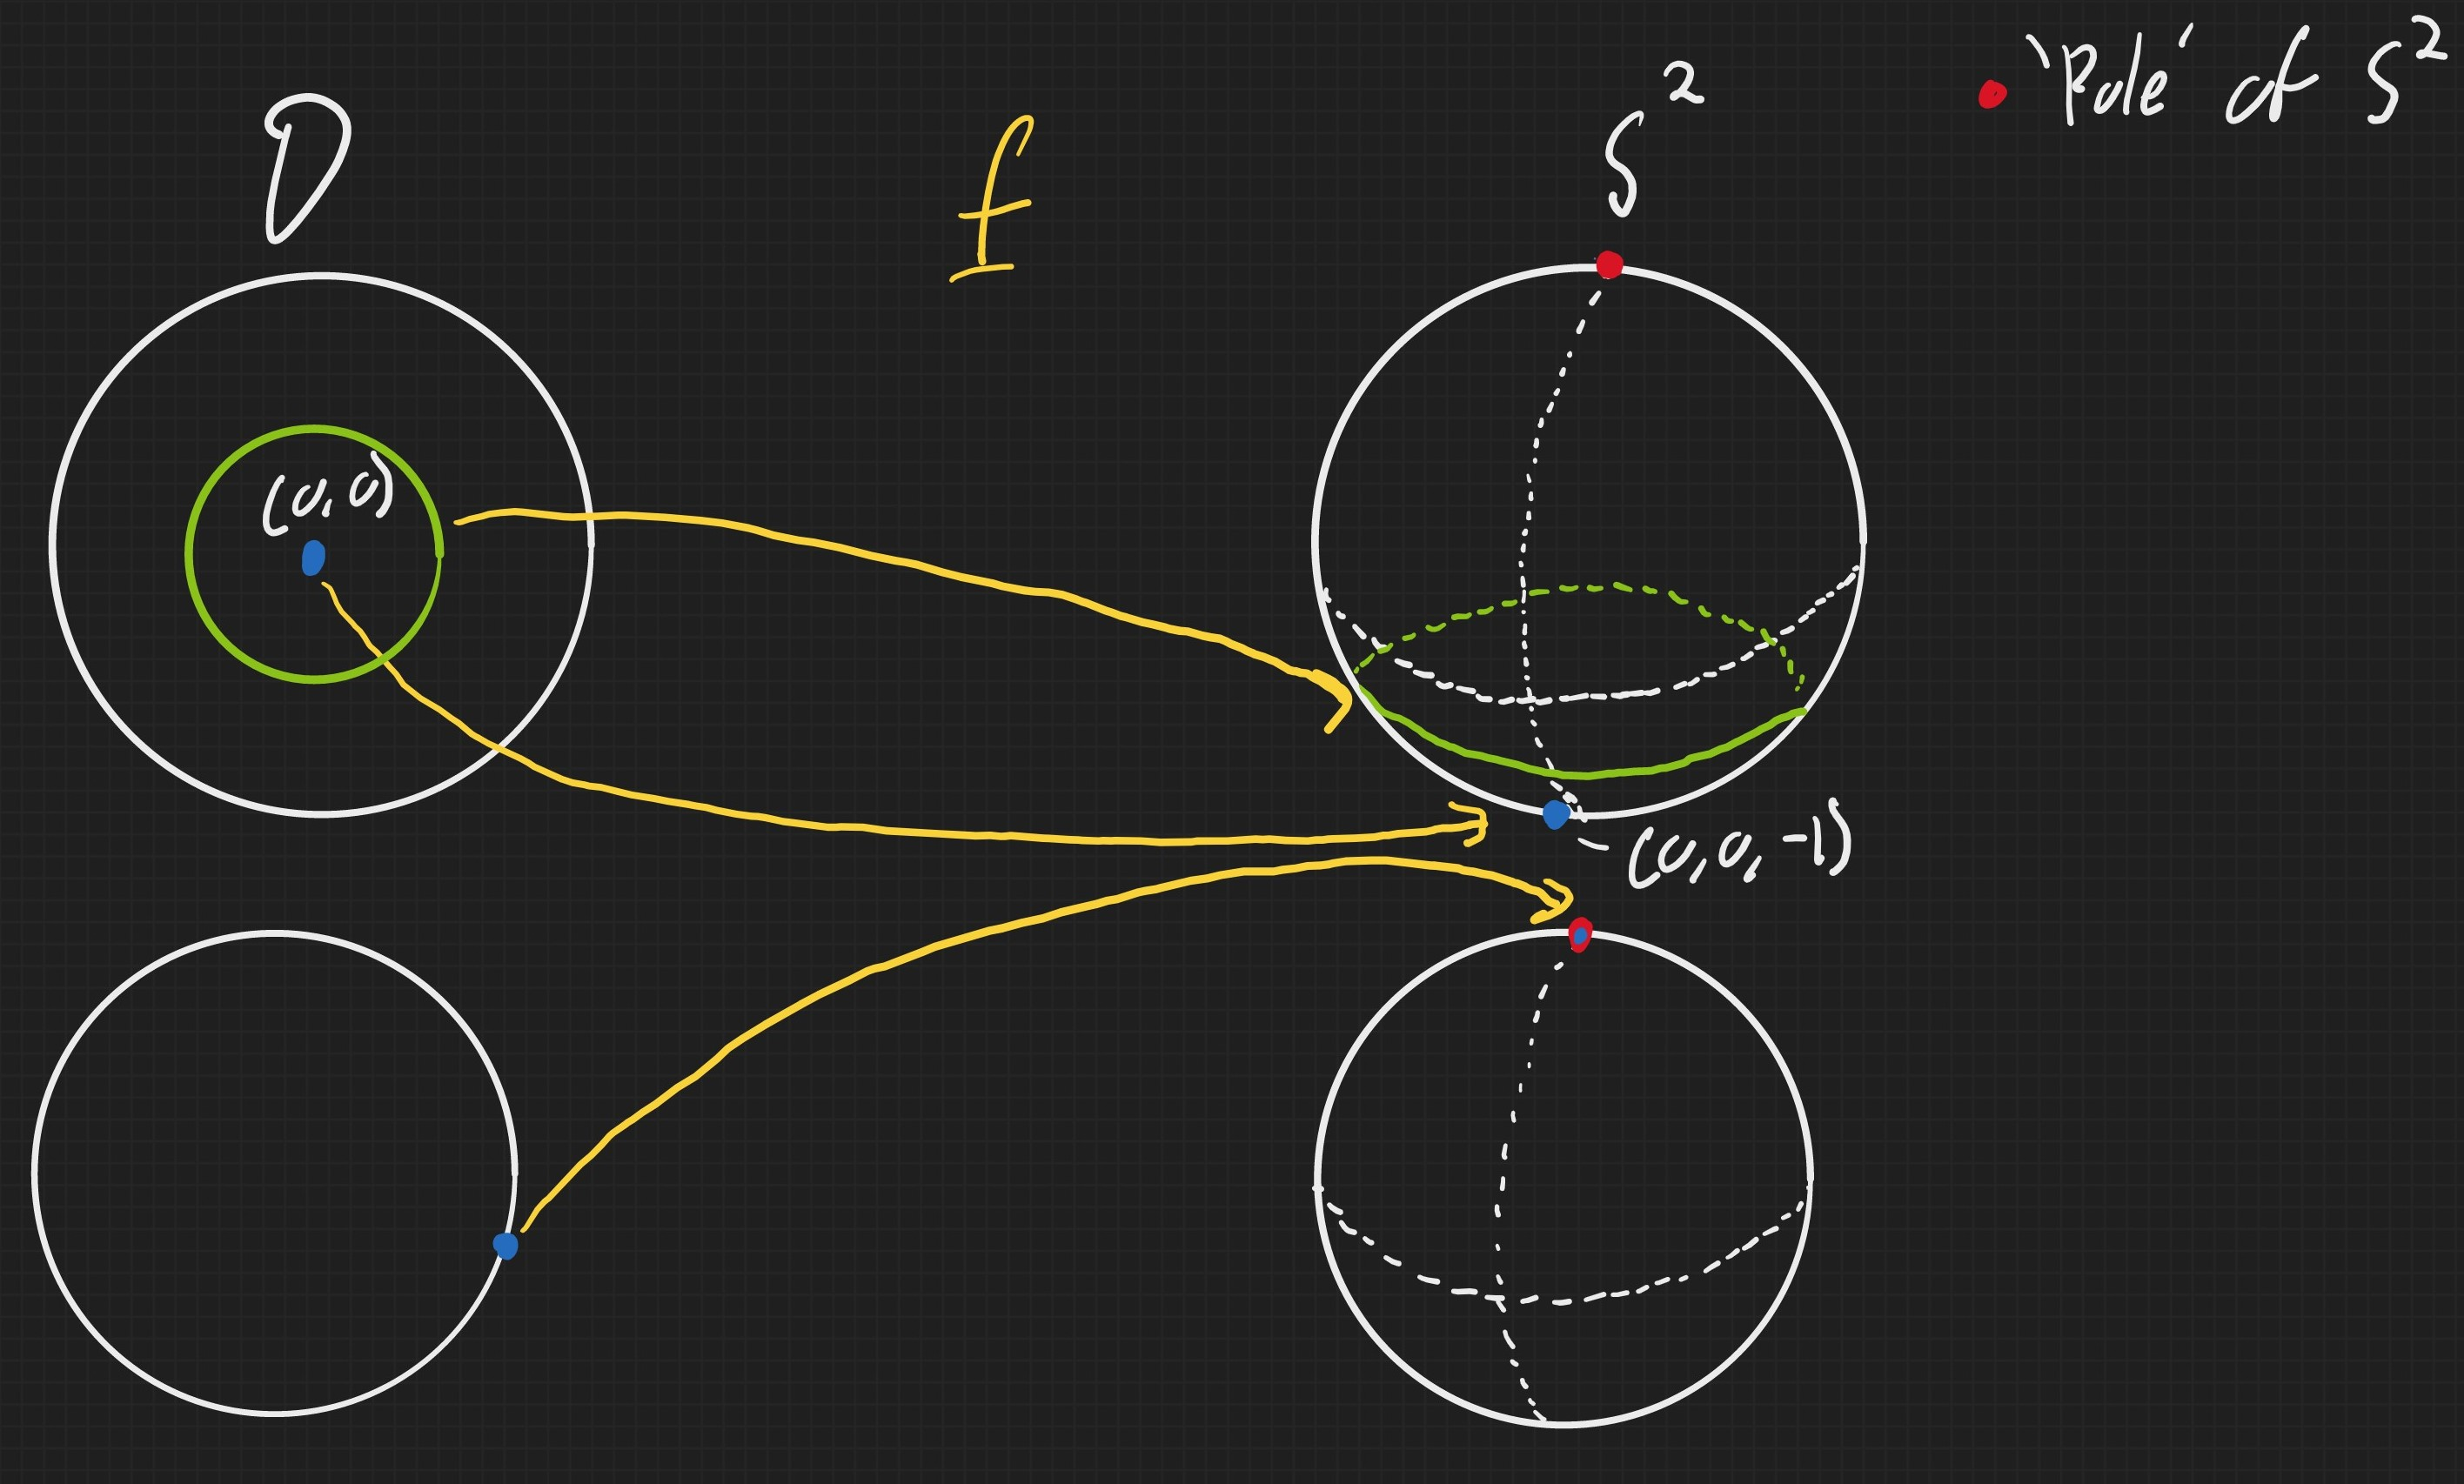
\includegraphics[scale=0.4]{ps7p222.JPG}
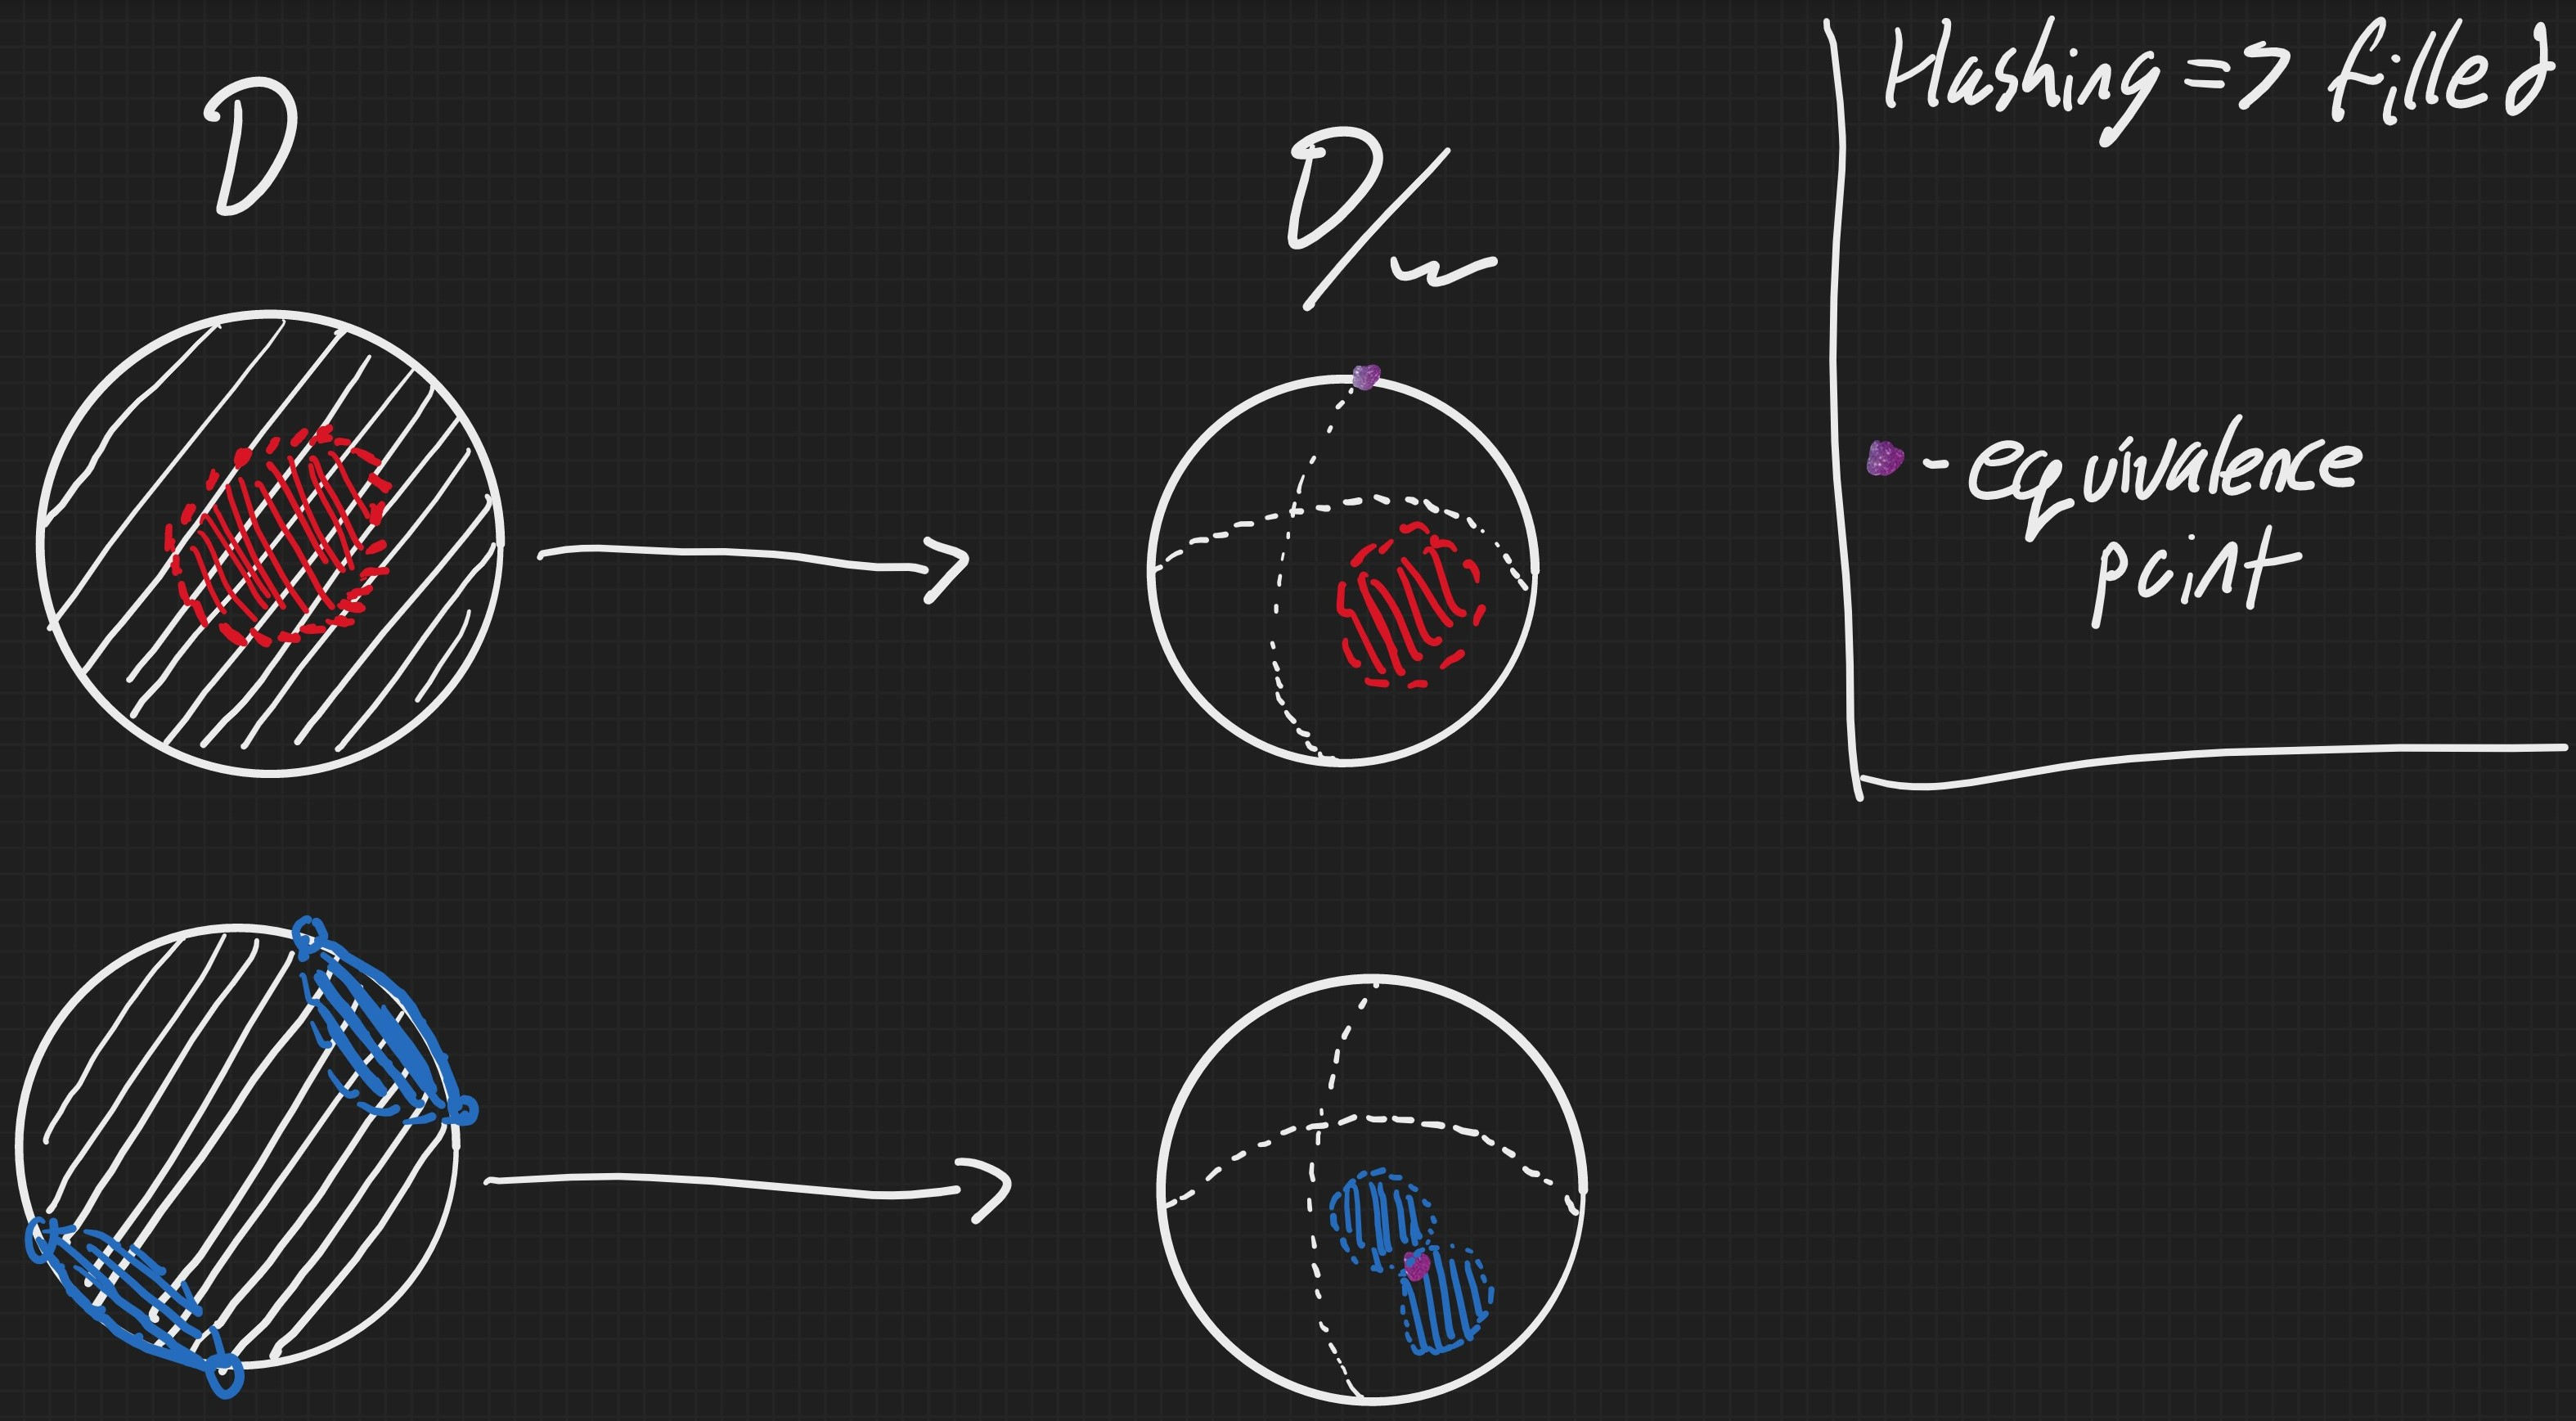
\includegraphics[scale=0.4]{ps7p2.JPG}
\end{center}

\item Let $X=X_1\times X_2\times \cdots \times X_n$ be a product of topological spaces. Define an equivalence relation $\sim$ on $X$ by declaring that $(x_1, x_2, \ldots,x_n)\sim (y_1,y_2,\ldots,y_n)$ if and only if $x_1 = y_1$. Show that $X/\sim$ is homeomorphic to $X_1$.\\\\
Let $\tau_1, \tau_2,\ldots, \tau_n$ be topologies on $X_1, X_2,\ldots, X_n$ respectively such that they are the topologies considered in $X$. Consider the function $f:X/\sim\rightarrow X_1$ defined by $f([(x_1, x_2,\ldots, x_n)])=x_1$. Now, let $[(x_1, x_2,\ldots, x_n)],[(y_1, y_2,\ldots, y_n)]\in X/\sim$ and assume that $f([(x_1, x_2,\ldots, x_n)])=f([(y_1, y_2,\ldots, y_n)])$. Then, $x_1=y_1$ and by definition, $(x_1, x_2, \ldots,x_n)\sim (y_1,y_2,\ldots,y_n)$. Hence $[(x_1, x_2, \ldots,x_n)]=[(y_1,y_2,\ldots,y_n)]$ and $f$ is injective. Now, let $x_1\in X_1$. Then there exists $[(x_1, x_2,\ldots x_n)]\in X/\sim$ such that $f([(x_1, x_2,\ldots, x_n)])=x_1$ by definition of $X$ and $X/\sim$. So, $f$ is also onto and therefore bijective. Now, let $U$ be an open set in $X_1$. Now, $(f\circ\nu)^{-1}(U)=\nu^{-1}(f^{-1}(U))$. Now, for every $(x_1, x_2,\ldots, x_n)\in\nu^{-1}(f^{-1}(U))$, we have that $(x_1, x_2,\ldots, x_n)\in U\times X_2\times\cdots\times X_n\subseteq\nu^{-1}(f^{-1}(U))$, and so $\nu^{-1}(f^{-1}(U))$ is open in $X$. Therefore, we have that $f$ is continuous. Now, let $U$ be an open set in $X/\sim$. So, $\nu^{-1}(U)$ is open in $X$. That is, for every $(x_1, x_2,\ldots, x_n)\in\nu^{-1}(U)$ there exists $V_1\times V_2\times\cdots\times V_n\in\tau_1\times\tau_2\times\cdots\times\tau_n$ such that $(x_1, x_2,\ldots, x_n)\in V_1\times V_2\times\cdots\times V_n\subseteq\nu^{-1}(U)$. Since, $f(U)=V_1$ and since $V_1$ is open in $X_1$, we have that $f$ is also an open map. Therefore, $f$ is a homeomorphism. Thus, $X/\sim\cong X_1$ as desired.

\item (\#1 in 5.5) A \textit{path} in a space $X_{\tau}$ is a continuous function $\alpha:[0,1]_{\mathcal{U}}\to X_{\tau}$. If $\alpha$ and $\beta$ are two paths in $X_{\tau}$ such that $\alpha(1) = \beta(0)$, then the map $\alpha \star \beta:[0,1]\to X$ defined by 
\[(\alpha \star \beta)(t)=\left\{ \begin{array}{ll}
                  \alpha(2t) & \mbox{$0\leq t\leq 1/2$}\\
                  \beta(2t-1)      & \mbox{$1/2 \leq t\leq 1$}
                  \end{array}
          \right. \]
 is continuous. (\textit{Hint}: Draw two such paths, then consider the Pasting Lemma.)\\\\
Let $X_{\tau}$ be a topological space and let $\alpha$ and $\beta$ be as given. Let $(\alpha\star\beta)$ be as stated above. Well, we have that $2t$ from $[0,\frac12]$ to $[0,1]$ and $2t-1$ from $[\frac12,1]$ to $[0,1]$ are both polynomials, and are therefore both continuous. Hence $\alpha(2t)$ and $\beta(2t-1)$ are both continuous. Now by the definition of $(\alpha\star\beta)$ above, define $A=[0,\frac12]$ and $B=[\frac12,1]$. We can seee that $A\cup B=[0,1]$, and $A$ and $B$ are both closed in $[0,1]$. Now, $A\cap B=\{\frac12\}$ and so $\alpha(2(\frac12))=\alpha(1)=\beta(0)=\beta(2(\frac12)-1)$ by definition. Thus, by the Pasting Lemma, we have that $(\alpha\star\beta)$ is continuous as desired.\\

 \item (\# 7a in 6.2) A space $X_{\tau}$ is said to be \textit{totally disconnected} if every subspace of $X$ with more than one element is disconnected (in the subspace topology). Show that every discrete space is totally disconnected.\\
Let $X$ be a set with the discrete topology. If $X$ itself has only one element, then $X_{\mathcal{D}}$ is vacuously totally disconnected. So, let $Card(X)\geq2$. Now, let $U$ be a subspace of $X_{\mathcal{D}}$ such that $Card(U)\geq2$. Then, consider the sets $V\subset U$ such that $V\neq\emptyset$ and $U\setminus V$. Hence $V, U\setminus V\neq\emptyset$, $V\cap(U\setminus V)=\emptyset$, and $V\cup(U\setminus V)=U$. Now, $V,(U\setminus V)$ are both open in the subspace topology, since $V$ and $(U\setminus V)$ are both open in $X_{\mathcal{D}}$, so $U$ is disconnected. Since $U$ was an arbitrary subspace with $Card(U)\geq2$, $X_{\mathcal{D}}$ is totally disconnected. Since $X_{\mathcal{D}}$ was also arbitrary, we have that every discrete space is totally disconnected as desired.



\end{enumerate}
\end{document}
